\documentclass[
	11pt,
]{beamer}

\newcommand\myheading[1]{%
  \par\bigskip
  {\Large\bfseries#1}\par\smallskip}


\graphicspath{{Images/}{./}} 

\usepackage{booktabs} 

%----------------------------------------------------------------------------------------
%	SELECT LAYOUT THEME
%----------------------------------------------------------------------------------------

\usetheme{CambridgeUS}

%----------------------------------------------------------------------------------------
%	SELECT COLOR THEME
%----------------------------------------------------------------------------------------

\usecolortheme{seahorse}

%----------------------------------------------------------------------------------------
%	SELECT FONT THEME & FONTS
%----------------------------------------------------------------------------------------

\usefonttheme{default} % Typeset using the default sans serif font

%------------------------------------------------

\usepackage{palatino} % Use the Palatino font for serif text

\usepackage[default]{opensans} % Use the Open Sans font for sans serif text

%----------------------------------------------------------------------------------------
%	SELECT INNER THEME
%----------------------------------------------------------------------------------------

\useinnertheme{circles}

%----------------------------------------------------------------------------------------
%	PRESENTATION INFORMATION
%----------------------------------------------------------------------------------------

\title[Parareal Algorithm]{\\ \textbf{Parareal Algorithm}}


\author[O. BOUHENNICHE \and N. ZAOUACHE]{Oussama BOUHENNICHE \and Narimane ZAOUACHE}

\institute[]{University of Strasbourg}


\date[\today]{ CSMI \\ \today}

%----------------------------------------------------------------------------------------

\begin{document}

%----------------------------------------------------------------------------------------
%	TITLE SLIDE
%----------------------------------------------------------------------------------------

\begin{frame}
	\titlepage
\end{frame}

%----------------------------------------------------------------------------------------
%	TABLE OF CONTENTS SLIDE
%----------------------------------------------------------------------------------------

\begin{frame}
	\frametitle{Presentation Overview}

	\tableofcontents
\end{frame}
%----------------------------------------------------------------------------------------
%	PRESENTATION BODY SLIDES
%----------------------------------------------------------------------------------------
\section{Context and objectives}

%------------------------------------------------
\begin{frame}
	\frametitle{Context and Objectives}
	\myheading{Context}
          study and implement the Parareal algorithm in sequential and in parallel and test it on lorenz system.

	\myheading{Objectives}

	\begin{columns}[c]
		\begin{column}{\textwidth}
			\begin{itemize}
                   \item study lorenz system and Implement Lorenz Model.
                   \item study the scipy.integrate package for ODEs solving and test it on lorenz system
                   \item study the Parareal algorithm and implement it in sequential
                   \item  study the parallelisation mechanism of the Parareal algorithm and implement it
               \end{itemize}
		\end{column}

	\end{columns}

\end{frame}

%------------------------------------------------
\section{The Lorenz system}

%------------------------------------------------
\begin{frame}
    \frametitle{The Lorenz system}

 The Lorenz system it can be described by the following three equations:
        \begin{figure}
                \includegraphics[width=1.\linewidth]{lorenz.png}
            \end{figure}
 
\end{frame}

%------------------------------------------------
\section{ODEs solvers}

%------------------------------------------------
\begin{frame}
    \frametitle{ODEs solvers}
    
       \begin{itemize}
           \item Euler Methods: a numerical techniques to approximate solutions of ordinary differential equations.
           
           \item Runge-Kutta Method is a more accurate and versatile family of numerical techniques for approximating ODE solutions.
           
           \item SciPy.integrate Package offers odeint and $solve_ivp$ functions for solving ODEs. 
       \end{itemize}
	
\end{frame}

%------------------------------------------------

\section{Parareal algorithm}

%------------------------------------------------
\begin{frame}
    \frametitle{Parareal algorithm}
    The algorithm works by dividing the time interval of interest into smaller subintervals and solving them concurrently using:
    \begin{columns}[c]
        \begin{column}{0.45\textwidth}
            \begin{itemize}
                \item The coarse solver provides a rough approximation of the solution over each subinterval.
                \item The fine solver refines this approximation to improve accuracy.
            \end{itemize}
        \end{column}
        \begin{column}{0.5\textwidth}
            \begin{figure}
                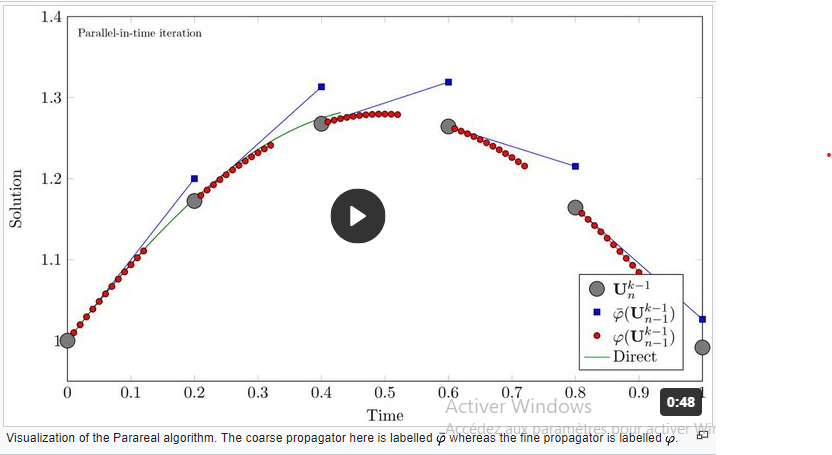
\includegraphics[width=1.\linewidth]{parareal.png}
            \end{figure}
        \end{column}
    \end{columns}
\end{frame}
%------------------------------------------------
   \begin{frame}
   \myheading{Parallelization}  
    The Parareal algorithm can be parallelized through domain decomposition, where the time domain is divided into subdomains assigned to different processors for the Parallel Fine Solver Application. Another approach involves utilizing dedicated frameworks for parallelization, such as Message Passing (for synchronizing computations and exchanging information between processors) and shared-memory or distributed-memory parallelism, like MPI or OpenCL.
   \end{frame}
%------------------------------------------------

\section{Numerical results}

%------------------------------------------------
\begin{frame}
	\frametitle{ Numerical results}
	\myheading{Lorenz chaotic phenomena: Sensitive dependence on the initial condition}
            \begin{column}{0.5\textwidth}
              \begin{figure}
                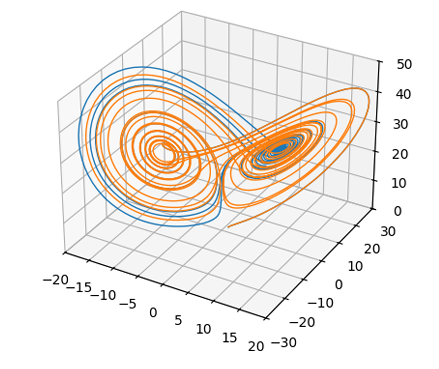
\includegraphics[width=1.\linewidth]{Lorenz_chaotic.png}
              \end{figure}
            \end{column} 

\end{frame}
%------------------------------------------------
   \begin{frame}
   \myheading{ Convergence check for Parareal algorithm on lorenz system}
            \begin{column}{0.5\textwidth}
              \begin{figure}
                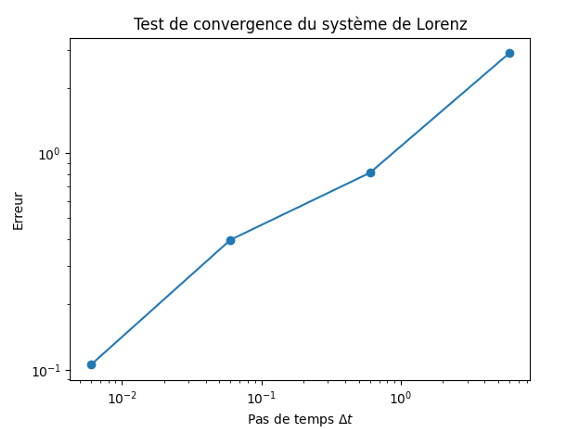
\includegraphics[width=1.\linewidth]{Convergence.png}
              \end{figure}  
            \end{column} 
   \end{frame}
%------------------------------------------------
   \begin{frame}
   \myheading{ Parareal performance comparison by the number of process}
            \begin{column}{0.5\textwidth}
              \begin{figure}
                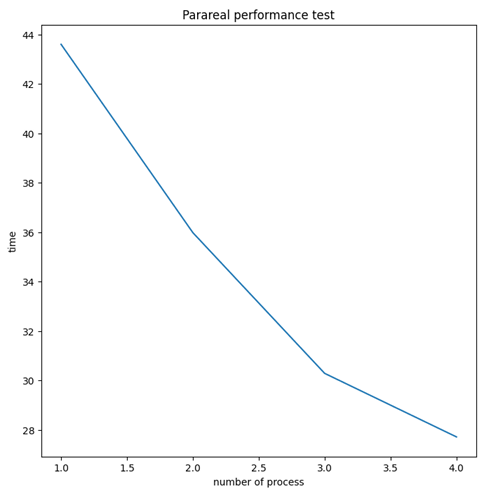
\includegraphics[width=1.\linewidth]{Parareal_perfo.png}
              \end{figure}  
            \end{column} 
   \end{frame}
%------------------------------------------------

\section{Conclusion}

%------------------------------------------------
\begin{frame}
	\frametitle{ onclusion}
	The ODE-solving methods discussed have unique strengths and weaknesses. While Euler, Runge-Kutta, odeint, and solve_ivp are sequential approaches suitable for many problems, the Parareal algorithm offers faster computation through parallelization, especially for precise solutions over extended time periods. Method selection depends on precision, computation speed, and implementation complexity. Future exploration could integrate Parareal's parallel computing advantage with the feel++ framework for solving PDEs.


\end{frame}


%------------------------------------------------




\section{References}

\begin{frame}[allowframebreaks]
	\frametitle{References}
	\bibliographystyle{plain}
	\bibliography{../References}
  \end{frame}

%------------------------------------------------

\begin{frame}
	\begin{center}
		{\Huge The End}

		\bigskip\bigskip

		{\LARGE Questions? Comments?}
	\end{center}
\end{frame}

%----------------------------------------------------------------------------------------


\end{document}